\section{Proximate Architecture and Programming Overview} \label{sec:arch}

This section first gives the architecture overview of proximate. Then
it details over how would one program proximate. And finally delve into the micro-arch details of
proximate.

\subsection{Architecture Overview}

\begin{figure}
  \begin{center}
    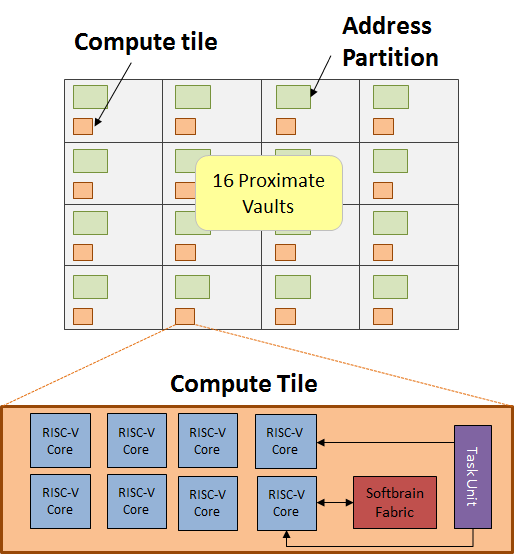
\includegraphics[width=0.65\linewidth, height=4.5in]{cs758-figs/arch-overview.png}
  \end{center}
\vspace{-0.2in}
  \caption{Proximate Architecture Overview}
  \label{fig:arch-overview}
\vspace{-0.05in}
\end{figure}

Figure~\ref{fig:arch-overview} shows the high level architecture organization of
proximate. As mentioned in Section~\ref{sec:motiv}, there is a vault abstraction 
in proximate with a compute substrate and an address partition. Proximate has 16 vaults, and this
decision is based on the bandwidth requirement of each vault and the interface to memory itself. 
The compute tile as shown in the detailed figures, further has 8 RISC-V~\cite{waterman2015risc}
cores for irregular computation and one Softbrain unit for regular workload acceleration. 
There is also a per-vault task unit responsible for offload the kernels and tracking their status
throughput the coarse of execution.

\subsection{Programming Overview}
We now explain how proximate would be programmed with the architecture overview 
described above. Figure~\ref{fig:prog-overview} shows how the original C/C++
program gets mapped to the proximate hardware components. The original C/C++ code
has 2 parts - i) The host code which has the proximate API calls (\emph{explained in detail in} Section~\ref{sec:prog}.)
to set up the memory, copy the memory
and en-queue the tasks, and ii) the second part is the actual computation kernel which gets offloaded to the compute tile
(\emph{shown in orange in figure}). The kernel portion of the program can have two parts again. If the programmer
identifies the computation as irregular workload, then that can be mapped to the in-order for energy efficient 
high concurrent execution. Whereas, if the kernel is a regular streaming workload, them it can be
mapped to the high-throughput engine \emph{Softbrain}. The task unit inside each compute unit is responsible for doing this mapping.  

\begin{figure}
  \begin{center}
    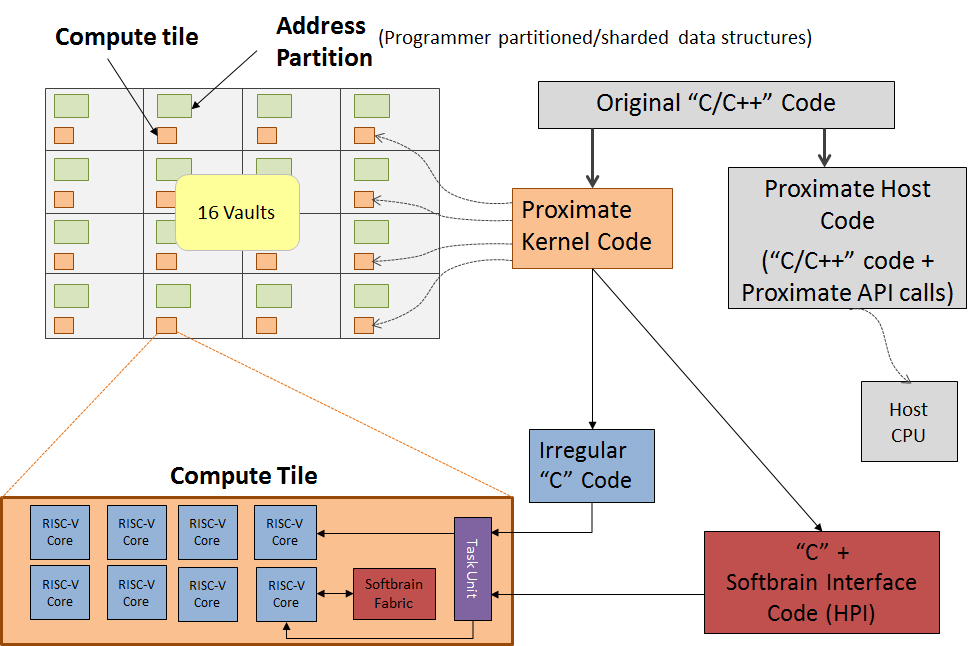
\includegraphics[width=\linewidth, height=4.5in]{cs758-figs/prog-overview.png}
  \end{center}
\vspace{-0.2in}
  \caption{Proximate Programming Overview}
  \label{fig:prog-overview}
\vspace{-0.05in}
\end{figure}

\subsection{Proximate Detailed Micro-Architecture}
Now, that we have understood both the architecture and programming overview of
proximate, this section details over the micro-architecture elements of proximate. 


\begin{figure}
  \begin{center}
    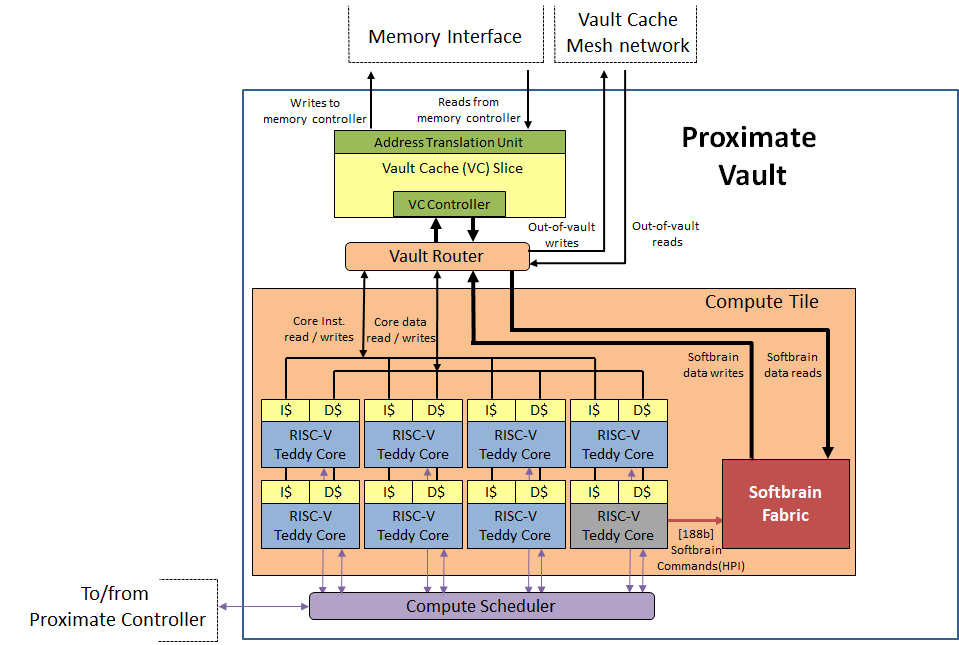
\includegraphics[width=\linewidth, height=4.5in]{cs758-figs/vault.png}
  \end{center}
\vspace{-0.2in}
  \caption{Proximate Vault Micro-Architecture}
  \label{fig:vault}
\vspace{-0.05in}
\end{figure}

Figure~\ref{fig:vault} shows the micro-architecture of each vault of proximate.
The compute tile part is same as the one described above in the arch. overview. The extra element is
the interface between one of the RISC-V cores and the Softbrain - \emph{command interface}.
Outside the compute tile is an address partitioned L2 cache or Vault Cache (VC) slice which is responsible
for handling all the memory requests from cores and softbrain. The vault router sitting in between the 
cache interface and compute tile is responsible for arbitration of many requests as well as
sending any out-of-vault access requests to global vault cache mesh network based on the address indexing the request is for.
Each vault also has a vault specific compute scheduler which is responsible for taking task requests from a global scheduler 
and offloading the tasks in each compute tile. The detailed design of this task based queuing model is described in Section~\ref{sec:queue}.

The high-throughput compute engine - Softbrain, is itself a big dataflow engine, and the details of
its micro-architecture are not described here as it is itself a big piece of design space to explore. 
Right now, one can assume each Softbrain unit has a Coarse-Grained Reconfigurable Architecture (CGRA) similar to Dyser~\cite{ieeemicro12:dyser}.
This CGRA has required mix of functional units to execute the kernel portion of regular workload. 


